
%%%%%%%%%%%%%%%%%%%%%%% file typeinst.tex %%%%%%%%%%%%%%%%%%%%%%%%%
%
% This is the LaTeX source for the instructions to authors using
% the LaTeX document class 'llncs.cls' for contributions to
% the Lecture Notes in Computer Sciences series.
% http://www.springer.com/lncs       Springer Heidelberg 2006/05/04
%
% It may be used as a template for your own input - copy it
% to a new file with a new name and use it as the basis
% for your article.
%
% NB: the document class 'llncs' has its own and detailed documentation, see
% ftp://ftp.springer.de/data/pubftp/pub/tex/latex/llncs/latex2e/llncsdoc.pdf
% Source URL: https://www.overleaf.com/9872043pgfkbjhyncvj#/36134551/
%%%%%%%%%%%%%%%%%%%%%%%%%%%%%%%%%%%%%%%%%%%%%%%%%%%%%%%%%%%%%%%%%%%


\documentclass[runningheads,a4paper]{llncs}

\usepackage{amssymb}
\setcounter{tocdepth}{3}
\usepackage{graphicx}
\usepackage{authblk}
\usepackage{lineno}
\usepackage{listings}
\usepackage[T1]{fontenc}

%\urldef{\mailsa}\path|{rtraborn, |
%\urldef{\mailsb}\path|vbrendel}@indiana.edu|    

\newcommand{\keywords}[1]{\par\addvspace\baselineskip
\noindent\keywordname\enspace\ignorespaces#1}

\begin{document}

\mainmatter  % start of an individual contribution

% first the title is needed
\title{Using RAMPAGE to identify and annotate promoters in insect genomes}

% a short form should be given in case it is too long for the running head
\titlerunning{Identification of insect regulatory elements}

% the name(s) of the author(s) follow(s) next
\author[1,2]{R. Taylor Raborn\thanks{Correspondence: rtraborn@indiana.edu}}
\author[1,2]{Volker P. Brendel}

\affil[1]{Department of Biology, Indiana University}
\affil[2]{School of Informatics and Computing, Indiana University}

%\date{\today}

\renewcommand\Authands{ and }
%
\authorrunning{Raborn and Brendel}
% (feature abused for this document to repeat the title also on left hand pages)

% the affiliations are given next; don't give your e-mail address
% unless you accept that it will be published
\institute{Department of Biology and School of Informatics and Computing, \\
Indiana University\\
212 S. Hawthorne Drive 205 Simon Hall, Bloomington, IN 47401, USA\\
%\mailsa\\
%\mailsb\\
\url{http://www.brendelgroup.org}}

%
% NB: a more complex sample for affiliations and the mapping to the
% corresponding authors can be found in the file "llncs.dem"
% (search for the string "\mainmatter" where a contribution starts).
% "llncs.dem" accompanies the document class "llncs.cls".
%

\toctitle{Lecture Notes in Computer Science}
\tocauthor{Authors' Instructions}
\maketitle


\begin{abstract}
Application of Transcription Start Site (TSS) profiling technologies, coupled with large-scale next-generation sequencing (NGS) has yielded valuable insights into the location, structure and activity of promoters across diverse metazoan model systems.
In insects, TSS profiling has been used to characterize the promoter architecture of \textit{Drosophila melanogaster} \cite{Hoskins:2011io}, and, shortly thereafter, to reveal widespread transposon-driven alternative promoter usage in \textit{D. melanogaster} \cite{Batut:2012kc}. 

In this chapter we highlight the utility of one TSS profiling method, RAMPAGE (RNA annotation and mapping of promoters for analysis of gene expression), for the precise, quantitative identification of promoters in insect genomes.
We demonstrate this using our tools GoRAMPAGE \cite{Brendel:2016ab} and TSRchitect \cite{Raborn:2017ab}, providing details instructions with the aim of taking the user from raw reads to processed results. 

\keywords{\textit{cis}-regulatory regions, promoter architecture, transcription initiation, transcription start sites (TSSs)}
\end{abstract}

\begin{linenumbers}
\section{Introduction}

\subsection{TSS Profiling Identifies Promoters at Genome-Scale}
The promoter, defined in eukaryotes as the genomic region bound by RNA Polymerase II immediately prior to transcription initiation \cite{Kadonaga:2011gz}, is the site where regulatory signals unite to direct gene expression.
The identification of promoter regions is a valuable step for understanding the \textit{cis}-regulatory signals that are present in an organism, and is also important for genome annotation.
However, despite the rapid accumulation of genome sequences across metazoan and arthropod diversity, accurate annotation of promoter regions remains sparse. 
This is because---absent empirically-defined information---precisely identifying sequence motifs that demarcate the promoter is unreliable.
In contrast with current \textit{in silico} approaches, direct mapping of TSSs identifies the location of the core promoter.
Cap Analysis of Gene Expression (CAGE) \cite{Kodzius:2006gy}, one of the first methods devised to identify 5$^\prime$-ends of mRNAs at large-scale, involves selective capture of 5$^\prime$-capped transcripts, first-strand reverse-transcription and ligation of a short oligonucleotide (CAGE tag). \\
\\
CAGE was initially utilized by the FANTOM (Functional Annotation of the Mammalian Genome) consortium to identify promoter architecture in human and mouse \cite{Carninci:2005kp}, providing the first glimpse of the global landscape of transcription initiation.
At the onset of the NGS era, CAGE was coupled with massively-parallel sequencing to generate 5`-ends of mRNAs at substantially higher scale. 
This advance provided more extensive coverage of the expressed transcriptome, and provided increased sensitivity for quantitative measurements \textit{i}.\textit{e}. measurement of promoter activity.

\subsection{Promoter Architecture of \textit{Drosophila melanogaster}}
Hoskins and colleagues \cite{Hoskins:2011io} performed CAGE in \textit{D. melanogaster} as part of the modENCODE consortium, identifying promoters at large-scale and characterizing the promoter architecture of an insect genome for the first time.
Hoskins \cite{Hoskins:2011io} indicated that TSS distributions at \textit{Drosophila} promoters exhibit a range of shapes that can be generally grouped into two major classifications: \textit{peaked} and \textit{broad}. 
Peaked promoters have a single, major TSS position occupying a narrow genomic region, whereas broad promoters lack a single, major TSS and contain TSSs across a wider region \cite{Rach:2009ct,Lenhard:2012en}. 
The authors also showed a strong association between promoter class and motif composition (consistent with previous findings \cite{Rach:2009ct,Ni:2010jh}). 
Peaked promoters were associated with positionally-enriched \textit{cis}-regulatory motifs including TATA, Initiator (Inr) and DPE, while broad promoters contained an enrichment of less-well characterized motifs, including \textit{Ohler6} and \textit{Ohler7} \cite{Ohler:2002vl}. 
The existence of two promoter classes appears to be conserved among metazoans, and has been reported (using TSS profiling methodolgies) in insects, cladocerans \cite{Raborn:2016cr}, fish \cite{Nepal:2013bga} and mammals \cite{Carninci:2006in,Lenhard:2012en}.

\subsection{Promoter Structure of Insects}
Beyond \textit{D. melanogaster}, few investigations have utilized TSS profiling in insect genomes. 
As a consequence, what is known about promoter architecture in insects is largely restricted to the \textit{Drosophila} genus. 
As part of the modENCODE effort, CAGE was performed in multiple tissues and developmental stages of the \textit{Drosophila pseudoobscura}. 
TSSs were found to be highly similar between species: more than 80\% of TSSs (81\%) of aligned, CAGE-identified TSSs from \textit{D. pseudoobscura} were positioned within 20nt of their counterparts in \textit{D. melanogaster}.
An enrichment of the CA dinucleotide was detected at the TSS ([-1, +1]), and the motifs corresponding to TATA, Inr and DPE were positioned at the same locations relative to the TSS in both species.
\\
\\
The only other insect species for which TSS profiling has been applied is the Tsetse fly (\textit{Glossina morsitans morsitans}) \cite{Mwangi:2015kn}. 
Using TSS-seq (specifically Oligo-capping; for details see \cite{Tsuchihara:2009dm}), the authors identified 3134 mapping to 1424 genes. 
The authors found a preference for CA and AA dinucleotides at the TSS, and observe the major core promoter elements observed in \textit{Drosophila}: TATA, Inr, DPE, in addition to MTE (Motif Ten Element).
As in \textit{D. melanogaster}, peaked promoters were more likely to contain TATA and Inr than broad promoters. 
While the taxonomic sampling of species for TSS profiling has been limited, the existing studies are sufficient to provide a general picture of insect promoter architecture.
A major demarcation between the promoter architecture of insects and mammals appears to be the large fraction of mammalian promoters found in CpG islands \cite{Mwangi:2015kn}.
CpG island promoters (CPIs) form the largest class of promoter in mammals \cite{Cvetesic:2017hl}; by contrast, CPIs are not known to exist as a class in invertebrates.


\subsection{Paired-end TSS Profiling with RAMPAGE}
The most recent major methodological advance in TSS Profiling is RAMPAGE (RNA Annotation and Mapping of Promoters for the Analysis of Gene Expression) \cite{Batut:2012kc,Batut:2013fu}. 
RAMPAGE is a protocol for 5$^\prime$-cDNA sequencing that combines cap trapping and template-switching with paired-end sequence information. 
A key advantage of generating paired-end sequence is transcript connectivity, which provides a direct link between a given 5$^\prime$-end and its associated mRNA molecule \cite{Batut:2012kc}.
Because short or spurious RNAs are found within the transcriptome, transcript connectivity allows the TSSs (and thus promoters) of full-length mRNAs to be unambiguously identified, which benefits genome annotation and improves interpretation of transcript species.
\\
\\
Batut and colleagues \cite{Batut:2012kc} generated libraries from total RNA isolated from 36 stages across the life cycle of \textit{D. melanogaster} providing a comprehensive gene expression and promoter atlas for fruit fly and in the process demonstrating the utility of RAMPAGE.
RAMPAGE is currently being applied as part of the latest iteration of ENCODE to identify promoters in human, but as of this writing it has not been applied to any non-\textit{Drosophila} insect model system. 
In anticipation of the future application of TSS profiling into other insect model systems here we provide a documented protocol for the computational processing RAMPAGE data, using selected libraries from Batut \textit{et al.} \cite{Batut:2012kc}. 
This method will consist of two parts: first, we will process, filter and align the sequenced RAMPAGE libraries to the \textit{D. melanogaster} genome. 
Second, we will identify TSSs and promoters from the aligned sequences and associate them with coding regions.
In closing, we will consider further applications of this data and discuss the utility of reproducible workflows in bioinformatic analysis.

%You are strongly encouraged to use \LaTeXe{} for the
%preparation of your camera-ready manuscript together with the
%corresponding Springer class file \verb+llncs.cls+. Only if you use
%\LaTeXe{} can hyperlinks be generated in the online version
%of your manuscript.

\section{Materials}

The analyses described herein require a workstation capable of doing modern bioinformatics, including a reasonably-appointed laptop.
An intermediate understanding of the Linux/Unix command line will be extremely useful, although we make efforts to explain the procedures with clarity. In addition, it will likely be necessary for the participant to have superuser privileges on the machine.
If you do not have a machine (or have access to one) that meets these requirements, it is recommended that you consider cloud-based cyberinfrastructure, including Amazon Web Services (AWS; \url{https://aws.amazon.com/}) or CyVerse (\url{http://www.cyverse.org/}) \cite{Merchant:2016jn}.
The former is a well-known pay-per-use solution, while the latter is an NSF-funded resource that makes compute allocations freely available to the public.

\subsection{Hardware}
\begin{enumerate} 
\item x86-64 compatible processors
\item At least 8GB RAM
\item 30GB+ hard disk space
\end{enumerate}

\subsection{Operating System}
\begin{itemize}
\item 64 bit Linux (preferred) or Mac OS X (with Command Line Tools from XCode)
\end{itemize}

\subsection{Software}
Below is a list of the software packages required for this demonstration (\textit{see} \textbf{Note 1}).\\
\\
\textbf{Sequence retrieval}
\begin{enumerate}
\item SRA Toolkit \cite{Leinonen:2011iw}  (\url{https://www.ncbi.nlm.nih.gov/sra/docs/toolkitsoft/})
\end{enumerate}
\textbf{GoRAMPAGE}
\begin{enumerate}
\item GoRAMPAGE \cite{Brendel:2016ab} (\url{https://github.com/brendelGroup/GoRAMPAGE})
\item fastq-multx \cite{Aronesty:2013gt} (\url{https://github.com/brwnj/fastq-multx})
\item FASTX-Toolkit \cite{citeulike:9103573} (\url{\texttt{http://hannonlab.cshl.edu/fastx\_toolkit/Index.html}})
\item TagDust2 \cite{Lassmann:2015gs} (\url{https://sourceforge.net/projects/tagdust/})
\item Samtools \cite{Li:2009ka} (\url{http://www.htslib.org/doc/samtools.html})
\item STAR \cite{Dobin:2016kq} (\url{https://github.com/alexdobin/STAR})
\end{enumerate}
\textbf{TSRchitect}
\begin{enumerate}
\item R (v. 3.4 and up) \cite{RCore:2017ab} (\url{https://www.r-project.org/})
\item Bioconductor (v. 3.5 and up) \cite{Lawrence:2014gy} (\url{http://bioconductor.org/})
\item TSRchitect \cite{Raborn:2017ab} (\url{http://bioconductor.org/packages/release/bioc/html/TSRchitect.html})
\item Various R package dependencies (see \textbf{Methods})
\end{enumerate}

\subsection{Online Appendix}
We created an online appendix to serve as a companion to this chapter, which contains both scripts and select files to assist you in completing this tutorial.
Please find the repository at \url{\texttt{https://github.com/rtraborn/MMB\_appendix}} (\textit{see} \textbf{Note 2}).

\subsection{Installation of R packages}
For installation of the software listed above, please follow the instructions provided by each respective package. 
Part of our analysis will require the use of R packages found in the Bioconductor suite \cite{Lawrence:2014gy}.
To install Bioconductor, please type the following from an R console: 

\noindent
\begin{verbatim}
source("https://bioconductor.org/biocLite.R")
biocLite()
\end{verbatim}

\noindent
We will use the R package \textit{TSRchitect} to identify promoters from aligned RAMPAGE libraries. 
Prior to running the analysis, it will be necessary to install a series of prerequisite packages to \textit{TSRchitect} from Bioconductor.
Please install these packages as follows (as before, from an R console):

\noindent
\begin{verbatim}
source("https://bioconductor.org/biocLite.R")
biocLite(c("AnnotationHub", "BiocGenerics", "BiocParallel",
 "ENCODExplorer",  "GenomicAlignments", "GenomeInfoDb",
 "GenomicRanges", "IRanges", "methods", 
 "Rsamtools", "rtracklayer", "S4Vectors",
 "SummarizedExperiment"))
\end{verbatim}

\noindent
To install \textit{TSRchitect}, please type the following from an R console:

\noindent
\begin{verbatim}
source("https://bioconductor.org/biocLite.R")
biocLite("TSRchitect")
\end{verbatim}

\noindent
Finally, please confirm that TSRchitect has been installed correctly by loading it from your R console as follows:

\noindent
\begin{verbatim}
library(TSRchitect) #installing TSRchitect
\end{verbatim}

\section{Methods}

\subsection{Retrieving the RAMPAGE sequence data from NCBI}

To begin our analysis, we must download the RAMPAGE data to our workstation. 
We will utilize tools provided by the SRA Toolkit, which should already be installed on your machine (see \textbf{Materials}).
The command \textit{fastq-dump} allows one to directly retrieve data from the GEO database using the appropriate identifier(s).
While there are 36 RAMPAGE libraries in the Batut \textit{et al.} paper, we will select a subset of these to analyze here.
We will compare samples from selected embryonic (E01h-E03h) and larval (L1-L3) tissues, representing the beginning and end of embryonic development.
For more information about the experiment and the available RAMPAGE libraries, please see the following link: \url{https://www.ncbi.nlm.nih.gov/Traces/study/?acc=SRP011193}.\\

\noindent
First, let's proceed with downloading the libraries from early embryonic tissues (\textit{see} \textbf{See Note 3}).
We will make a new folder (entitled \texttt{"fastq\_files/"}) to house these files.

\noindent
\begin{verbatim}
mkdir fastq_files
cd fastq_files

fastq-dump --split-files SRR424683
fastq-dump --split-files SRR424684
fastq-dump --split-files SRR424685
\end{verbatim}

\noindent
We continue by downloading the data from late larval tissues.

\begin{verbatim}
fastq-dump --split-files SRR424707
fastq-dump --split-files SRR424708
fastq-dump --split-files SRR424709
\end{verbatim}

\noindent
Once the download of the aforementioned files are complete, you should see a total of 12 (6 \textit{x} 2) separate fastq files in your current working directory:

\noindent
\begin{verbatim}
ls -l *.fastq | wc -l
cd ..
\end{verbatim}

\subsection{Creating symlinks to the files}
Our workflow expects fastq files that have the format ``*.R1/R2.clipped.fq". 
Rather than rename them, we can simply create brand new symbolic links (symlinks) to the files, as follows:

\noindent
\begin{verbatim}
cd ..
mkdir -p output/reads/clipped
cd output/reads/clipped

#embryonic libraries
ln -s ../../../fastq-files/SRR424683_1.fastq E01h.R1.clipped.fq 
ln -s ../../../fastq-files/SRR424683_2.fastq E01h.R2.clipped.fq
ln -s ../../../fastq-files/SRR424684_1.fastq E02h.R1.clipped.fq
ln -s ../../../fastq-files/SRR424684_2.fastq E02h.R2.clipped.fq
ln -s ../../../fastq-files/SRR424685_1.fastq E03h.R1.clipped.fq
ln -s ../../../fastq-files/SRR424685_2.fastq E03h.R2.clipped.fq

#larval libraries
ln -s ../../../fastq-files/SRR424707_1.fastq L1.R1.clipped.fq 
ln -s ../../../fastq-files/SRR424707_2.fastq L1.R2.clipped.fq
ln -s ../../../fastq-files/SRR424708_1.fastq L2.R1.clipped.fq
ln -s ../../../fastq-files/SRR424708_2.fastq L2.R2.clipped.fq
ln -s ../../../fastq-files/SRR424709_1.fastq L3.R1.clipped.fq
ln -s ../../../fastq-files/SRR424709_2.fastq L3.R2.clipped.fq

cd ../../.. #returning to the output directory
\end{verbatim}

\subsection{Downloading genomic data from \textit{D. melanogaster}}
Now that we have the fastq files from the RAMPAGE libraries downloaded and named appropriately, we now must retrieve the genome assembly and rRNA sequences from \textit{D. melanogaster}.
The genome assembly is required for aligning the RAMPAGE reads, and the rRNA sequences are required to filter out matching reads in the sequenced RAMPAGE libraries, since our sample is intended to contain only capped RNA transcripts. 
Please download the rRNA sequences from the link we provide below. 
These sequences were retrieved separately from Genbank at the NCBI database. \\

\noindent
To retrieve the genome assembly from the ENSEMBL database, please do the following:

\noindent
\begin{verbatim}
mkdir genome
cd genome
wget ftp://ftp.ensembl.org/pub/release-78/fasta/drosophila_melanogaster/dna/Drosophila_melanogaster.BDGP5.dna.toplevel.fa.gz
#uncompressing the file
gzip -d Drosophila_melanogaster.BDGP5.dna.toplevel.fa.gz
cd ..
\end{verbatim}

\noindent
Please navigate to the rRNA file \texttt{"Dmel\_rRNA.fasta"} found in the Appendix.

\noindent
\begin{verbatim}
head -n 3
>ref|NR_133562.1| Drosophila melanogaster 28S ribosomal RNA (28SrRNA:CR45844), rRNA
TTATATACAACCTCAACTCATATGGGACTACCCCCTGAATTTAAGCATATTAATTAGGGGAGGAAAAGAA
ACTAACAAGGATTTTCTTAGTAGCGGCGAGCGAAAAGAAAACAGTTCAGCACTAAGTCACTTTGTCTATA
\end{verbatim}

\subsection{Filtering and alignment of RAMPAGE reads using GoRAMPAGE}
At this stage we are ready to commence with the rRNA filtering and alignment of the RAMPAGE libraries.
We will use GoRAMPAGE, a tool we developed, to perform these tasks in a concerted workflow. 
GoRAMPAGE runs TagDust \cite{Lassmann:2015gs} to remove rRNA and low-complexity reads, and uses STAR \cite{Dobin:2016kq} to align RAMPAGE (or other paired-end) reads to a given genome assembly.

\subsubsection{Setting up the GoRAMPAGE job.}
Please refer to the script \texttt{"GoRAMPAGE\_script\_MMB.sh"} and (using a text editor) provide the appropriate paths to the genome assembly, output directory (see above) and rRNA sequences (\textit{see} \textbf{Note 4}). 
GoRAMPAGE jobs can optionally be run in parallel (\textit{see} \textbf{Note 5}).
The script can be executed as follows:

\noindent
\begin{verbatim}
#vi GoRAMPAGE_script_MMB.sh #updating with a text editor
./GoRAMPAGE_script_MMB.sh
\end{verbatim}

\noindent
If everything is working correctly you should start to see the results of the job being written to the file "errScript".
You can inspect the progress during the run using the \textit{less} command. 

\noindent
\begin{verbatim}
less -S errScript
\end{verbatim}

\noindent
Should the run fail before completion, any associated error messages will be printed to the errScript file. Once the job is complete, you should see the message "GoRAMPAGE job is complete!" appear on the command-line terminal.

\subsubsection{Inspecting the rRNA filtering results.}

To evaluate the results from Step 3 (rRNA filtering), please navigate to the top level of the "output" directory and open the file "LOGFILES".
You'll see the recorded progress of the program Tagdust and a record of the results.
We notice that (for the L3h library) 1046448 of reads (78.1\%) were "extracted", meaning that slightly more than 20\% of reads were removed because of matches with ribosomal sequences.
The removed reads from all libraries are found in the \texttt{"dusted\_discard"} directory, and the extracted reads are found in the current directory. 
Due to their sheer abundance within cells, ribosomal RNA sequences are an inevitable contaminant within TSS profiling libraries. 
For analysis purposes, it is important that these sequences be removed, which is what has been completed here.\\
Since this step was conducted appropriately, we can proceed to the next step.

\subsubsection{Evaluating the alignments.}

The folder "alignments/" in your GoRAMPAGE output folder will now contain 6 .bam files, each representing the distinct RAMPAGE libraries selected for our analysis.
Typing "ls -l" from the command line will show that these files are symlinks to the original alignment files found in the "STARoutput/" directory.
"STARoutput/", as its name suggests, contains the output from the STAR alignment, and this includes the alignment files "*.sortedByCoord.out.bam", and four additional log files.
The files with the suffix "*.STAR.Log.final.out" each contain a summary of the alignment, such as the number of input reads, the percentage of uniquely-mapped reads and the percentage of unmapped reads.
An inspection of these log files indicates that the alignments have similar mapping rates (~70-80\%), a reasonable outcome for our purposes.\\

\noindent
Now that our RAMPAGE libraries are filtered and aligned, we can commence with the second half of our analysis.

\subsection{Promoter identification from aligned RAMPAGE libraries}

We can now use the prepared alignment files to identify TSSs and promoters from the selected RAMPAGE libraries.
There are currently several tools available for this purpose.
\textit{CAGEr}, developed by Haberle \cite{Haberle:2015fp}, was utilized to perform TSS identification as part of the FANTOM5 efforts.
We will use \textit{TSRchitect} in this demonstration, since it was specifically designed to analyze paired-end TSS profiling datasets, and also because it is more flexible with respect to model system (\textit{i.e.} it does not require a corresponding \textit{BSGenome} package).
The latter feature will be helpful when analyzing the non-\textit{D. melanagaster} TSS profiling datasets that we expect to be generated in the near future.

\subsubsection{Setting up the Analysis.}
\textit{TSRchitect}, the package we'll use for this analysis, is an R package available in the Bioconductor suite of genomics tools \cite{Lawrence:2014gy}.
It makes use of existing packages and data structures within this environment, where available, to identify promoters from sequence alignments.
Since you have already installed \textit{TSRchitect} and its dependencies (see section 2.3), we are set to proceed.\\
\\
There are two general ways one can choose to run \textit{TSRchitect}. 
The first is interactively \textit{i.e.} typing the instructions directly into an R console.
While this is a perfectly acceptable way to run analyses using package, for larger jobs it will likely be more efficient (and likely more reproducible) to run a dedicated R script.
We have provided a sample script \texttt{"MMB\_chapter\_TSRchitect.R"} to make it easier for you to set up an R script. 
In the section to follow, we will go through the output of the analysis. 
For further details on how to use \textit{TSRchitect}, please see its documentation at its Bioconductor page found here: \url{https://www.bioconductor.org/packages/release/bioc/html/TSRchitect.html}.\\

\subsubsection{Running the Analysis.}
To run TSRchitect using the batch script, provide full paths for the variables "BAMDIR" and "DmAnnot" in the script provided (\textit{see} \textbf{Note 6}).
\textit{BAMDIR} should be a path to the subdirectory "alignments/" in RAMPAGE output directory you specified earlier, and \textit{DmAnnot} should be a full path to the \textit{D. melanogaster} gene annotation listed above.\\
\\
Once this is complete, we can run the batch script from the Linux command-line as follows:

\noindent
\begin{verbatim}
R CMD BATCH MMB_chapter_TSRchitect.R
#assumes variables BAMDIR and DmAnnot have already been set
bg #puts this job in the background
\end{verbatim}

\noindent
Once the job is underway, you can monitor its progress by looking at the contents of the .Rout file (in this case, \texttt{"MMB\_chapter\_TSRchitect.Rout"}). 
The job should complete within an hour on most systems.\\

\subsubsection{Reviewing the \textit{TSRchitect} script.} 
Before we evaluate the results (which will have been written to your working directory after running the batch script), there are some important aspects of the analysis to review. 
We discuss these for informational purposes only; it will not necessary to perform these commands separate from the batch script provided.
First, we must initialize the \textit{tssObject} (which stores the information about the experiment) appropriately (\textit{see} \textbf{Note 7}).\\

\noindent
The inputs in this case are BAM files (\textit{inputType}="bam"); \textit{TSRchitect} also accepts input in BED format.

\noindent
\begin{verbatim}
DmRAMPAGE <- loadTSSobj(experimentTitle = "RAMPAGE Tutorial", \
 inputDir=BAMDIR, inputType="bam", isPairedEnd=TRUE, \
 sampleNames=c("E1h","E2h", "E3h", "L1", "L2", "L3"), \
 replicateIDs=c(1,1,1,2,2,2))
\end{verbatim}

\noindent
A critical step in our analysis is identifying TSRs from the aligned TSS data; to do this we use the function \textit{determineTSR}. 
We have selected the job to run on 4 cores in this example (\textit{n.cores}=4). 
Please enter the number of cores appropriate for your system.
Because we want to identify TSRs from every one of the selected RAMPAGE libraries, we specify \textit{tssSet}="all".
The parameter \textit{tagCountThreshold} was set to 25, meaning that only TSSs supported by 25 or more 5$^\prime$ RAMPAGE reads will be included within a TSR.
Setting \textit{writeTable} to "TRUE" means that the identified TSRs from each set will be written to the working directory. 

\noindent
\begin{verbatim}
DmRAMPAGE <- determineTSR(experimentName=DmRAMPAGE, n.cores=4, \
 tsrSetType="replicates", tssSet="all", tagCountThreshold=25, \
 clustDist=20, writeTable=TRUE)
\end{verbatim}

\textit{TSRchitect} can incorporate the tag abundances from each of the samples and append them to the list of identified TSRs. 
This is useful for downstream analysis of differential expression.

\noindent
\begin{verbatim}
DmRAMPAGE <- addTagCountsToTSR(experimentName=DmRAMPAGE, \
tsrSetType="replicates",  tsrSet=1, tagCountThreshold=10, \
 writeTable=TRUE)
\end{verbatim}

We can use \textit{TSRchitect} to import an annotation file (or, alternatively, use an existing one from \textit{AnnotationHub}) and use it to associate our set of identified TSRs with coding genes. 
We can specify the maximum distances (both up- and downstream) between the TSR and the annotation using the arguments \textit{upstreamDist} and \textit{downstreamDist}.

\noindent
\begin{verbatim}
DmRAMPAGE <- importAnnotationExternal(experimentName=DmRAMPAGE, \
 fileType="gff3",  annotFile=DmAnnot)

DmRAMPAGE <- addAnnotationToTSR(experimentName=DmRAMPAGE, \
 tsrSetType="replicates", tsrSet=1, \
upstreamDist=1000, downstreamDist=200, feature="gene", \
 featureColumnID="ID", writeTable=TRUE)
\end{verbatim}

Now we have generated a set of identified TSSs, TSRs from all 6 RAMPAGE libraries, and have associated the identified TSRs with annotated genes. 
Next, we will merge the libraries into two samples according to condition: early embryonic (E1h, E2h, E3h) and late larval (L1, L2, L3) using the information we provided when we initialized the \textit{tssObject} at the start of this section.
After merging, we identify promoters i) within the merged samples and ii) within the entire dataset combined, and associate with the \textit{D. melanogaster} gene annotation as described previously (not shown).

\noindent
\begin{verbatim}
#merging the sample data into two groups
DmRAMPAGE <- mergeSampleData(DmRAMPAGE)

# ... identifying TSRs from the merged samples:
DmRAMPAGE <- determineTSR(experimentName=DmRAMPAGE, \
n.cores=4, tsrSetType="merged", \
 tssSet="all", tagCountThreshold=40, \
 clustDist=20, writeTable=TRUE)
\end{verbatim}

\subsubsection{Evaluating the results}
Our analysis using \textit{TSRchitect} is now complete.
Your working directory should now contain the following: 
\begin{itemize}
\item TSSs from each sample \textit{e.g.} TSSset-1.txt: (6)
\item TSRs from each sample (in both .txt and .tab formats): (12)
\item TSRs from each merged group (in both .txt and .tab formats): \textit{e.g.} TSRsetMerged-1.txt: (4)
\item TSRs from the combined set of TSSs: TSRsetCombined.tab: (1)
\end{itemize} \\

\noindent
Let's briefly review the files (\textit{see} \textbf{Note 8}). 
We can quickly obtain the counts on the command line, as follows:

\noindent
\begin{verbatim}
wc -l *.tab
8377 TSRset-1.tab
6159 TSRset-2.tab
4814 TSRset-3.tab
17924 TSRset-4.tab
11851 TSRset-5.tab
3242 TSRset-6.tab
13986 TSRsetCombined.tab
7344 TSRsetMerged-1.tab
12126 TSRsetMerged-2.tab
85823 total
\end{verbatim}

\noindent
We will see that we have identified between roughly 3,200 and 18,000 TSRs within the individual RAMPAGE samples, which is attributable to the differences in library sizes. 
We detect 7,344 TSRs within the early embryonic samples ("TSRsetMerged-1.tab") and 12,126 TSRs in the late larval samples ("TSRsetMerged-2.tab").
Within the combined samples ("TSRsetCombined.tab") we find 13,986 TSRs, which is similar to the number reported by Hoskins \textit{et. al.} \cite{Hoskins:2011io}.\\

\noindent
In addition to identifying the position of a given TSRs, \textit{TSRchitect} records other useful information about its properties.
The \textit{width} of a TSR refers the span of the genomic region it occupies (in bp), and the \textit{Shape Index} (SI) is measure of the relative peakedness of the TSR.
We can see an example of this in the file "TSRsetMerged-1.txt".

\noindent
\begin{verbatim}
seq     start   end     strand  nTSSs   tsrWidth        shapeIndex      featureID
2L.67043.67044.+        2L      67043   67044   +       270     2       1       NA
2L.74089.74115.+        2L      74089   74115   +       341     27      0.13    NA
2L.94739.94752.+        2L      94739   94752   +       1650    14      0.55    FBgn0031216
2L.102386.102386.+      2L      102386  102386  +       284     1       2       FBgn0031217
\end{verbatim}

\subsection{Summary}
The workflow provided here is intended to serve as a useful entry point for the analysis of TSS profiling data in insects. 
On the computational side, we have provided an open source set of tools so that the uninitiated genome scientist can begin to analyze RAMPAGE (or other forms of TSS profiling data) quickly.
While the analysis centered on \textit{D. melanogaster} via the use of public datasets, it is anticipated that this will assist groups who may be interested in performing TSS profiling in their preferred insect model system.The application of TSS profiling technology across a more representative sample of insect diversity will improve our understanding of the positions and general structure \textit{cis}-regulatory regions in this phylum.

\subsection{Figures}

\begin{figure}
\centering
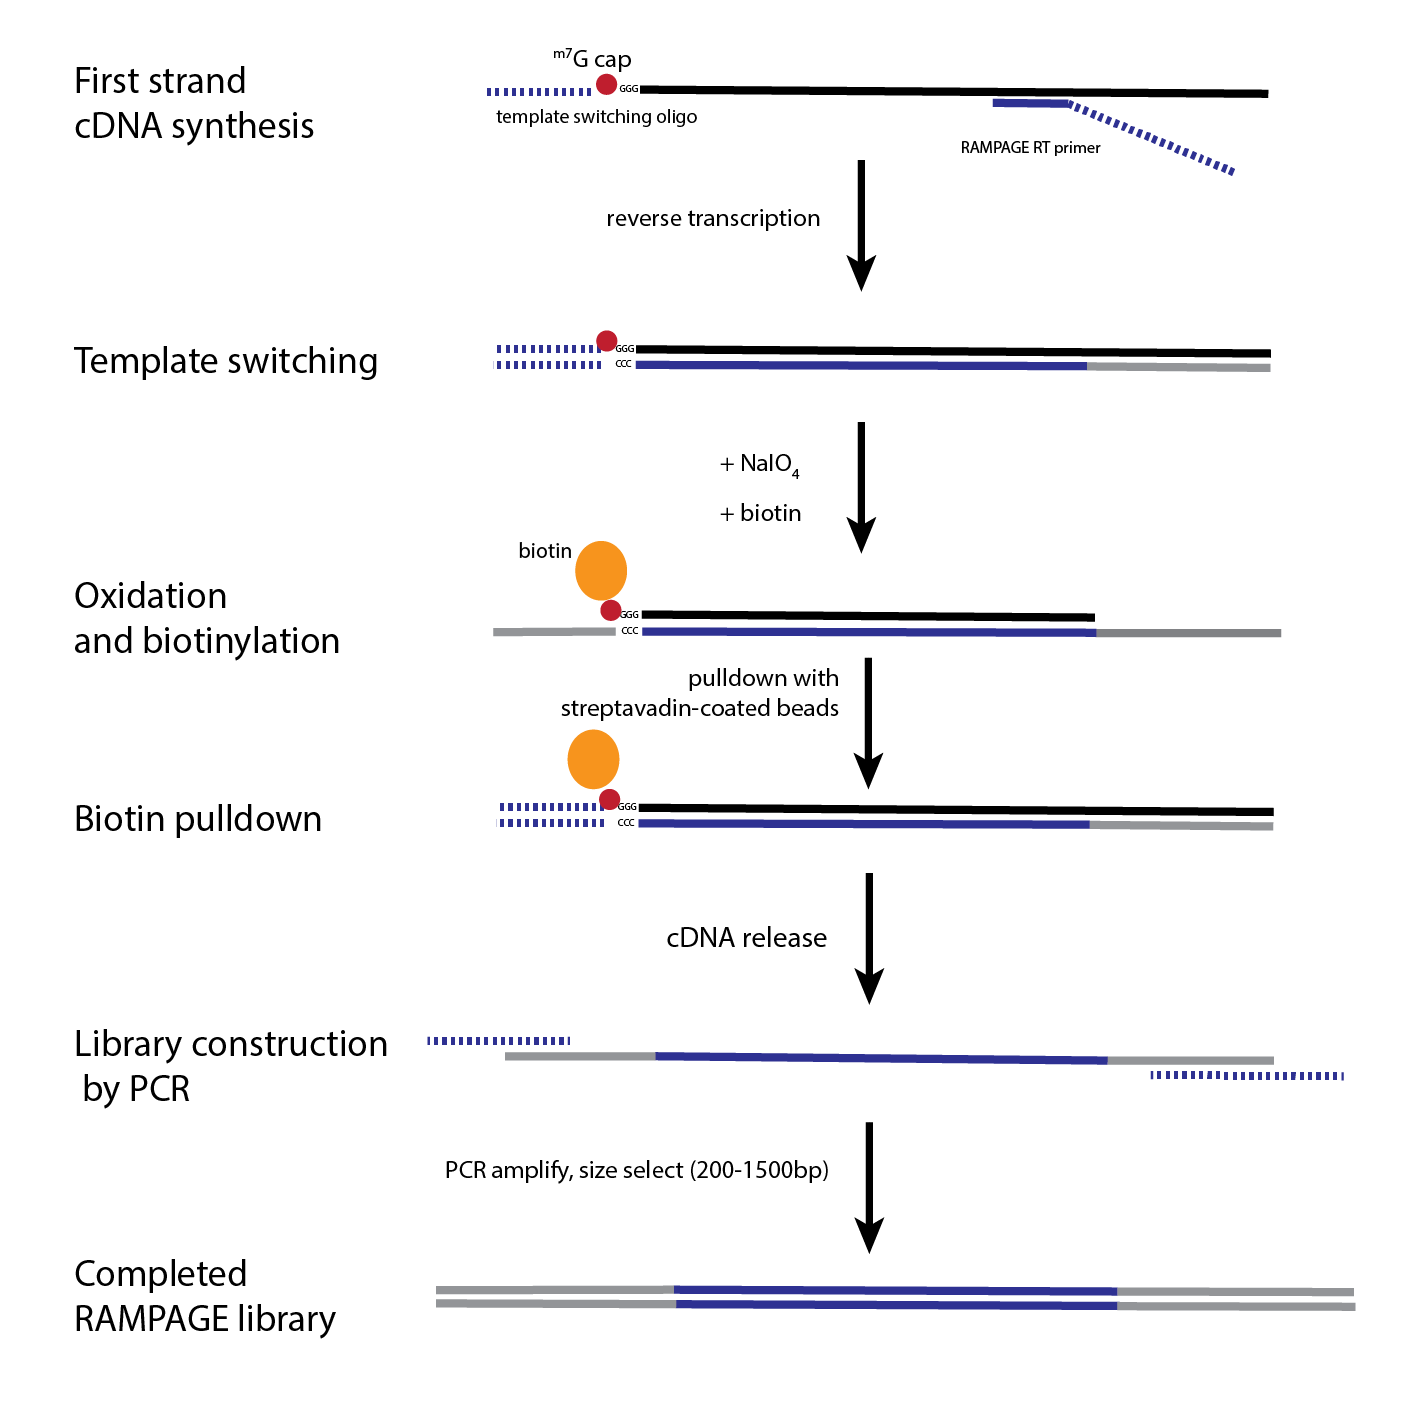
\includegraphics[height=15cm]{Figures/Insect_Chapter_Figure_1}
\caption{A brief summary of the RAMPAGE protocol. Starting with high-quality total RNA, first-strand cDNA synthesis is initiated using a cap-bound oligonucleotide and a custom RAMPAGE RT primer, creating a double-stranded DNA-RNA hybrid molecule. Next, the 5$^\prime$-m7G cap is oxidized, bound with biotin and pulled down with streptavadin-coated beads. The single-stranded cDNA molecules is released and the final RAMPAGE library construction is completed with PCR using custom oligonucleotides, followed by size-selection. This illustration was adapted from \cite{Batut:2013fu}.}
\label{fig:figure1}
\end{figure}

\begin{figure}
\centering
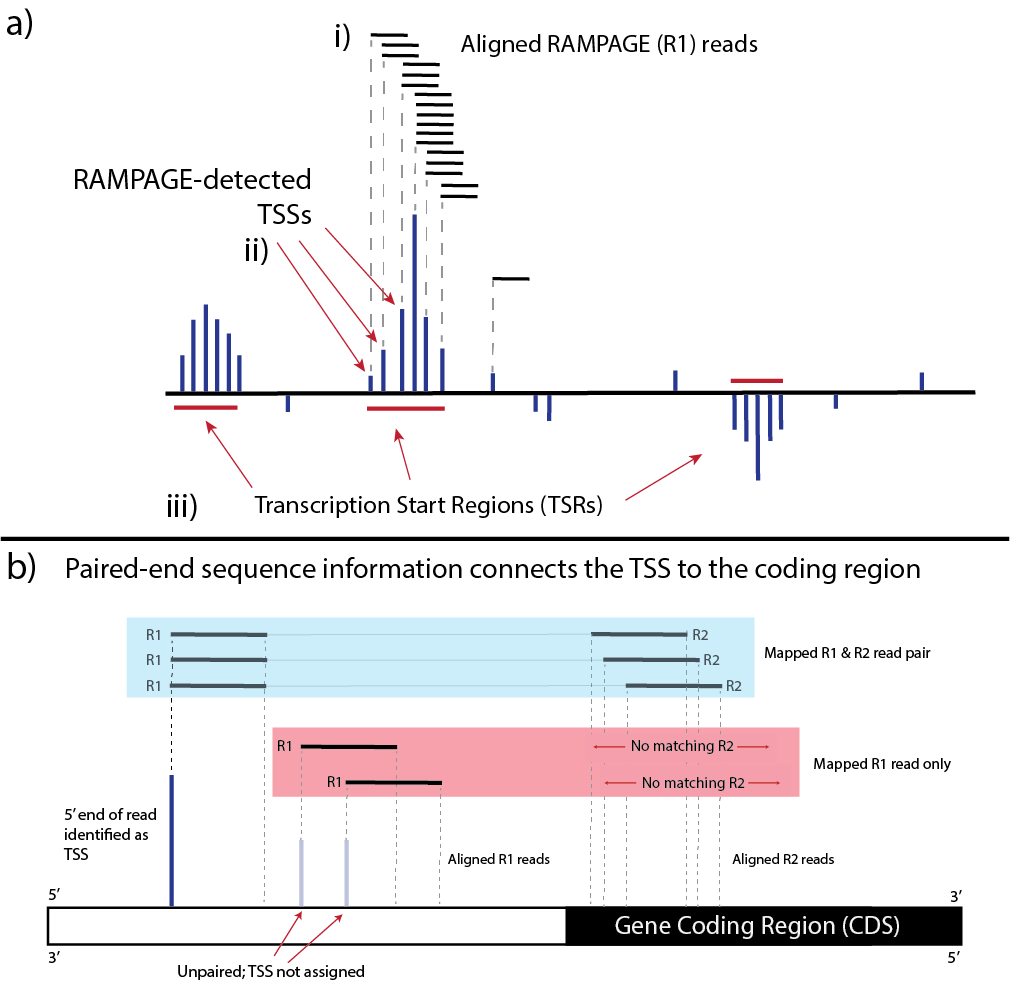
\includegraphics[height=7cm]{Figures/Insect_Chapter_Figure_2.png}
\caption{An overview of promoter identification using RAMPAGE. a) RAMPAGE reads are aligned to the genome. The 5$^\prime$-most genomic coordinate from each properly-paired R1 read is estimated as a TSS. The ambundance of mapped 5$^\prime$-ends at a given TSS is a measure of its abundance. TSSs above a minimum threshold will be clustered into TSRs. b) RAMPAGE-derived Paired-end sequence information provides a connection between a 5$^\prime$-mRNA end and a gene coding region. Only properly-paired R1 reads (\textit{i.e.} with an aligned R2 read) are identified as TSSs and then included in the downstream clustering procedure described in part \textit{a}.}
\label{fig:figure2}
\end{figure}

\begin{figure}
\centering
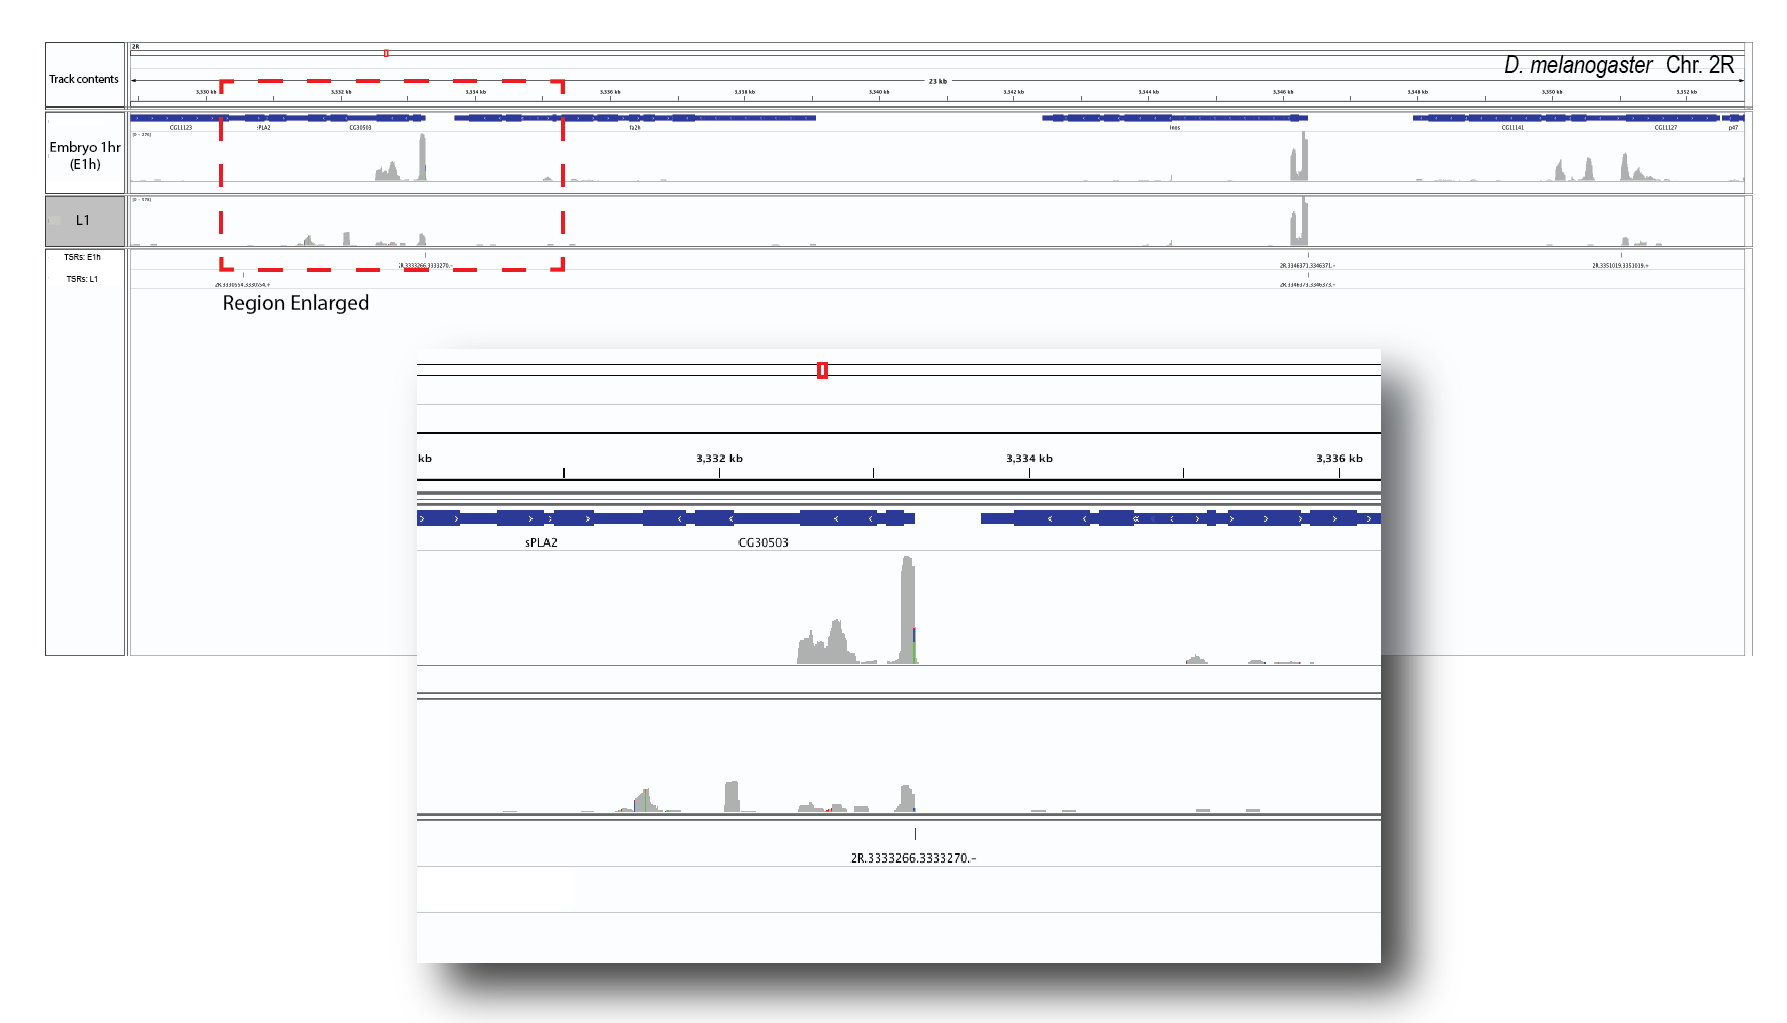
\includegraphics[height=8.65cm]{Figures/Insect_Chapter_Figure_3.png}
\caption{Test caption for Figure 3}
\label{fig:figure3}
\end{figure}

\section{Notes}
\begin{enumerate}
\item Please consult the GoRAMPAGE documentation found here:\\
 \url{https://github.com/BrendelGroup/GoRAMPAGE}.\\
Installation instructions for the prerequisites of GoRAMPAGE (which includes some of the items listed) are found at the following link:\\
 \url{https://github.com/BrendelGroup/GoRAMPAGE/tree/master/src}.
\item You can clone this appendix to your workspace on the command line using git, as follows:
\begin{verbatim}
git clone https://github.com/rtraborn/MMB_appendix.git
\end{verbatim}
The "scripts/" folder in the Appendix contains code for you to run the two major workflows described in this chapter.
The "\texttt{additional\_files/}" folder contains the following files which are necessary for the analysis: i) a fasta file containing ribosomal RNA sequences for \textit{D. melanogaster} (\texttt{Dmel\_rRNA.fasta}) and ii) a gene annotation for \textit{D. melanogaster} (\texttt{Drosophila\_melanogaster.BDGP5.78.gff}).
\item Since these fastq files are paired-end, we use the argument \textit{--split-files} to generate separate files for each read pair.
\item If you are running this on a cluster with a job scheduler you'll need to add the necessary headers to the top of the script and submit the job in the appropriate manner.
\item For parallel execution, GoRAMPAGE uses the Linux package \textit{GNU parallel} \cite{Tange2011a}. 
Please see the GoRAMPAGE documentation for more information.
\item To do this, please edit the batch script \texttt{TSRchitect\_script\_MMB.R} with a text editor of your choice.
\item Because the samples provided derive from related developmental stages, we will merge them for annotation purposes using the argument \textit{replicateIDs}, (though it must be emphasized that they are not replicates).
\item All of \textit{TSRchitect's} output files are labeled according to the order that they are loaded onto the \textit{tssObject}. 
For example, \textit{TSSset-1.txt} corresponds to the first RAMPAGE dataset (in our case E1h), and \textit{TSSset-2.txt} corresponds to the second RAMAPGE dataset (for this example E2h), and so on.
You can check which datasets are loaded on the \textit{tssObject} by simply entering it on an R console. 
Please see the \textit{TSRchitect} documentation for more information.

\subsection*{Acknowledgments}
The authors would like to thank Philippe Batut for generous technical assistance with the RAMPAGE protocol, and to Nathan Keith for his help establishing the protocol in our laboratory.

\subsection*{Disclosure Declaration}
The authors declare that they have no competing interests.
\end{linenumbers}

\section{References}\label{references}

% if your bibliography is in bibtex format, use those commands:
\bibliographystyle{IEEEtran} % Bibliography style file
\bibliography{RAMPAGE_chapter}      % Bibliography file

\section{Checklist of Items to be Sent to Volume Editors}
Here is a checklist of everything the volume editor requires from you:

\begin{itemize}
\settowidth{\leftmargin}{{\Large$\square$}}\advance\leftmargin\labelsep
\itemsep8pt\relax
\renewcommand\labelitemi{{\lower1.5pt\hbox{\Large$\square$}}}

\item The final \LaTeX{} source files
\item A final PDF file
\item A copyright form, signed by one author on behalf of all of the
authors of the paper.
\item A readme giving the name and email address of the
corresponding author.
\end{itemize}
\end{document}
